This section presents a simulation analysis of the evaluative network. Recall that the generative-evaluative architecture (GEA) comprises both the generative model (GM) and the evaluative model (EM). We can evaluate aspects of these separately. After training, the EM was used to predict grasp outcomes in the test set. This comprised 1,241 scenes with 76,213 grasps. Of these, 40,243 succeeded and 35,970 failed. Our analysis is given in Table~\ref{fig:predictions}. The sensitivity is 0.84 and the specificity 0.71. The F1-score is 0.802.
\begin{table}[b]
\centering
\caption{Confusion matrix for prediction on simulated data.}
\label{fig:predictions}
\begin{tabular}{|c|c|c|c|c|c|}
\hline
 & & \multicolumn{4}{c|}{Prediction} \\ \cline{3-6}
      & & \multicolumn{2}{c|}{\#} & \multicolumn{2}{c|}{\%} \\ \cline{3-6}
  &  & Succ         & Fail         & Succ         & Fail         \\ \hline
\multirow{ 2}{*}{Ground Truth} \newline & Succ & 33890      & 6353       & 84\%     & 16\%       \\ \cline{2-6}
 &Fail & 10339      &  25631    & 29\%     &  71\%   \\ \hline
\end{tabular}
\end{table}
% In this context, precision is the fraction of correctly labeled grasps among those predicted to be of a certain class (success or failure). Recall stands for the fraction of relevant grasps that have been identified correctly among all grasps that belong to that class. The results show a high recall rate for successful grasps, and there are relatively more false positives than false negatives. This necessitates pairing our evaluative neural network with a generative model rather than a random grasp generator, which would likely result in very low quality grasps and consequently, more false positives. 

%To test our generative-evaluative learning architecture we compared the grasp it proposes to the grasp proposed by the generative learner alone. Since \citet{kopicki2015ijrr} showed a 77.7\% success rate with the original generative algorithm we generated a new test set that contained both more challenging objects and placed them in challenging poses. The difficulty single-view grasping with a depth camera depends greatly on the pose of the object relative to the camera. The set comprised 40 test objects (Figure~\ref{fig:real-objects}) and another six training objects. The training objects were used by the human to demonstrate ten example grasps (Figure~\ref{fig:generative-training}). The 40 test objects were used to generate 49 object-pose pairs. From the 40 objects, 35 belonged to object classes in the simulation dataset, while the remaining five do not. 

\begin{figure}[t]
  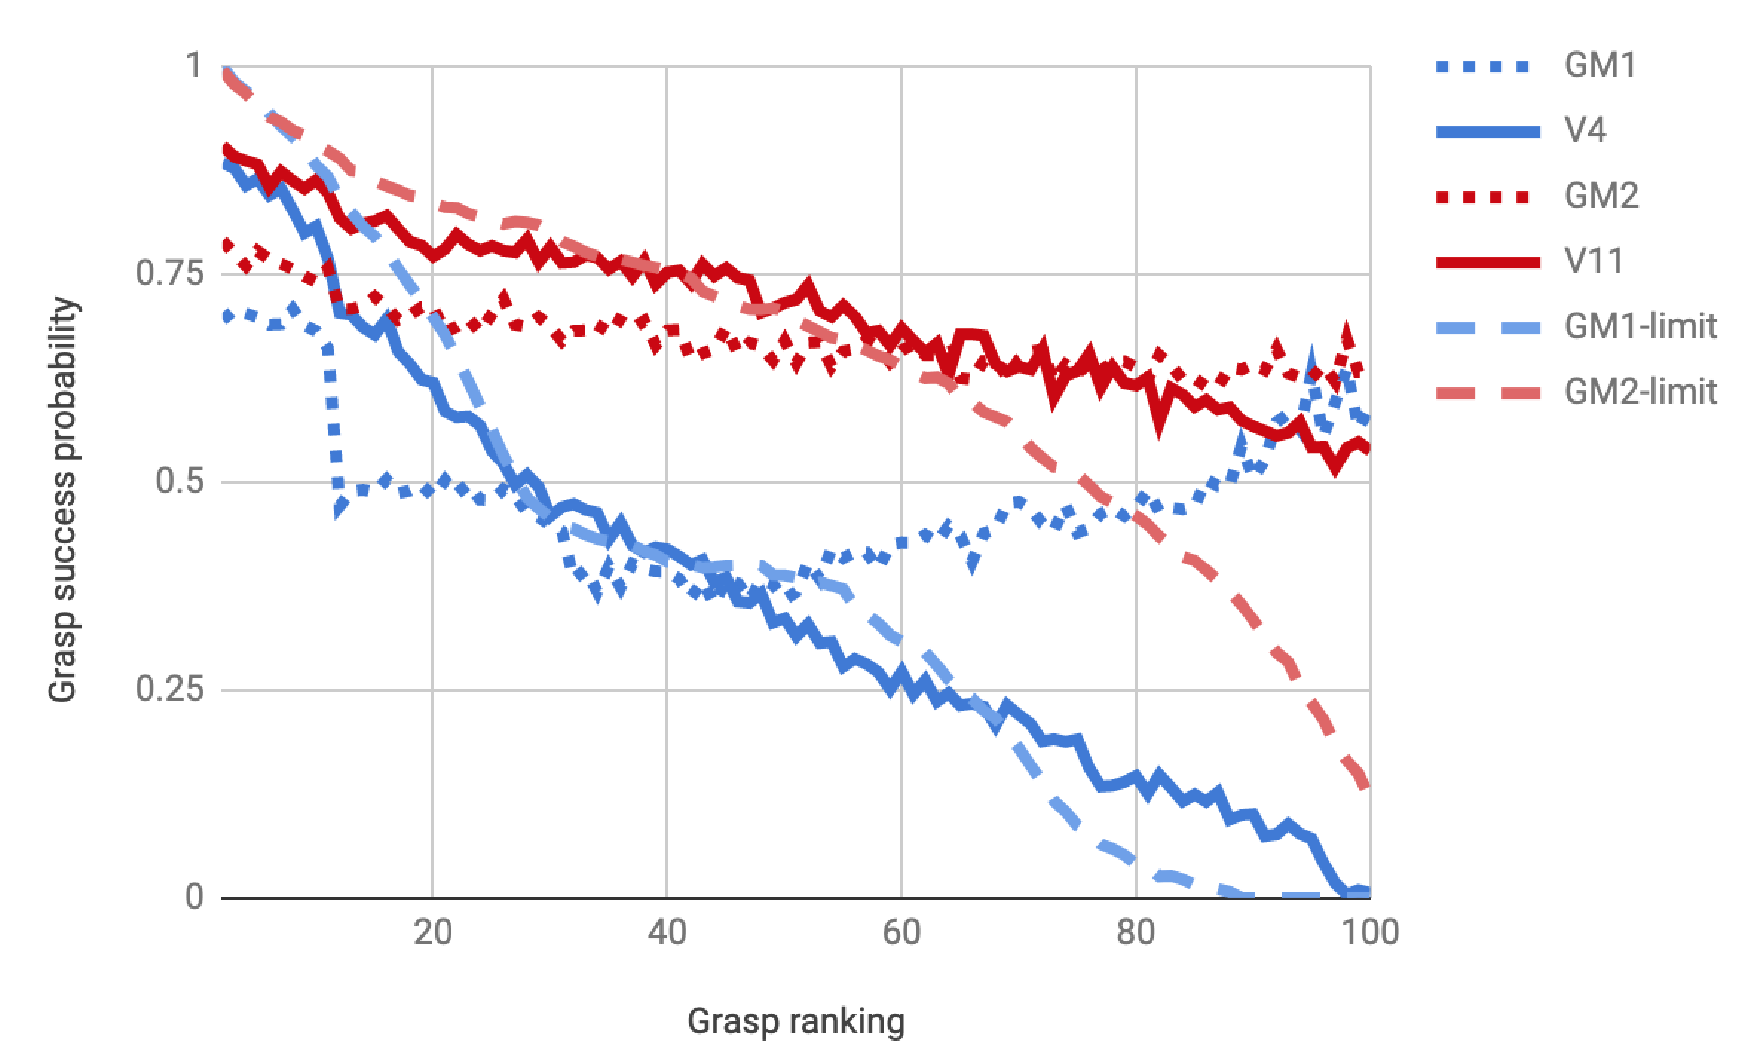
\includegraphics[width=\linewidth]{images/successvsranking.pdf}
  \caption{Grasp success probability (in simulation) vs. grasp ranking.}
  \label{fig:successvsranking}
\end{figure}

We compared the EM and GM rankings (Figure~\ref{fig:successvsranking}). The x-axis shows the ranking. The y-axis shows the average actual success rate over all scenes (1,241 test, 7,311 training). When ranked by the EM, the grasp success probability falls nearly monotonically, as is desirable. On the other hand, the likelihood-based ranking of GM results in many good grasps being low-ranked. We also wish to know whether the grasps recommended by the EM and the GM have different grasp success rates. The success rates of the top-ranked grasps are 71.59\% (GM) and  84.2\% (EM).

We also investigated using the EM to improve grasps directly. Lu et al. \cite{lu2017planning} proposed gradient ascent on the input grasp parameters to the EM with respect to the predicted success probability. They initialised with a heuristic grasp. We initialise with the best grasp proposed by the GEA. We ran 20 and 100 epochs of gradient ascent on the EM network inputs. Although predicted success rate rises, the success rate in simulation declines. After 20 epochs it is 1.3\% lower and after 100 epochs it is 4.8\% lower than the actual success rate of the initial grasp. This suggests that optimising dexterous grasps by the EM is non-trivial, perhaps because of the high-dimensionality of the grasp space. We speculate that initialising with a random grasp would be even worse.

%A pure generative model architecture (GM) and the generative-evaluative architecture (GEA) were evaluated using a paired trials methodology. Each was presented with the same object-pose combinations. Each architecture generated a ranked list of grasps, and the highest ranked grasp was executed. The highest-ranked grasp based on the predicted success probability of the network is performed on each scene. A grasp was deemed successful if, when lifted for five seconds, the object then remained stable in the hand for a further five seconds before being automatically released. The success rate for GM was 57.1\% and for GEA it was 77.6\%. The successes and failures for each method were recorded and are summarised in Table~\ref{tab:robot-results}. A two-tailed McNemar test, for the difference between success rates for paired comparison data, was performed and the difference between the two algorithms has a $p$-value of 0.0442, and so is statistically significant. A selection of grasps where the two methods performed differently are shown in Figure~\ref{fig:successfail}.

% OLD TABLE
%\begin{table}
%\begin{center}
%\caption{Results of the real robot paired comparison trial.}
%\begin{tabular}{|c|c|c|c|}  \hline 
%          &                & \multicolumn{2}{ c |}{ GM} \\ \hline
%          &                & \# succs & \# fails  \\  \hline
 %GEA  & \# succs &  23 &  15  \\
 %         & \# fails    &  5   &   6   \\ \hline
%\end{tabular}
%\end{center}
%\label{tab:robot-results}
%\end{table}

%Training parameters for network. Training of example grasps for learning from demonstration. Creation of real test data set. Paired comparisons methodology with vanilla LFD algorithm (pose + object + camera view).
%
%The actual grasping tests have been performed on the real robot. 